\documentclass[twoside]{book}

% Packages required by doxygen
\usepackage{fixltx2e}
\usepackage{calc}
\usepackage{doxygen}
\usepackage[export]{adjustbox} % also loads graphicx
\usepackage{graphicx}
\usepackage[utf8]{inputenc}
\usepackage{makeidx}
\usepackage{multicol}
\usepackage{multirow}
\PassOptionsToPackage{warn}{textcomp}
\usepackage{textcomp}
\usepackage[nointegrals]{wasysym}
\usepackage[table]{xcolor}

% Font selection
\usepackage[T1]{fontenc}
\usepackage[scaled=.90]{helvet}
\usepackage{courier}
\usepackage{amssymb}
\usepackage{sectsty}
\renewcommand{\familydefault}{\sfdefault}
\allsectionsfont{%
  \fontseries{bc}\selectfont%
  \color{darkgray}%
}
\renewcommand{\DoxyLabelFont}{%
  \fontseries{bc}\selectfont%
  \color{darkgray}%
}
\newcommand{\+}{\discretionary{\mbox{\scriptsize$\hookleftarrow$}}{}{}}

% Page & text layout
\usepackage{geometry}
\geometry{%
  a4paper,%
  top=2.5cm,%
  bottom=2.5cm,%
  left=2.5cm,%
  right=2.5cm%
}
\tolerance=750
\hfuzz=15pt
\hbadness=750
\setlength{\emergencystretch}{15pt}
\setlength{\parindent}{0cm}
\setlength{\parskip}{3ex plus 2ex minus 2ex}
\makeatletter
\renewcommand{\paragraph}{%
  \@startsection{paragraph}{4}{0ex}{-1.0ex}{1.0ex}{%
    \normalfont\normalsize\bfseries\SS@parafont%
  }%
}
\renewcommand{\subparagraph}{%
  \@startsection{subparagraph}{5}{0ex}{-1.0ex}{1.0ex}{%
    \normalfont\normalsize\bfseries\SS@subparafont%
  }%
}
\makeatother

% Headers & footers
\usepackage{fancyhdr}
\pagestyle{fancyplain}
\fancyhead[LE]{\fancyplain{}{\bfseries\thepage}}
\fancyhead[CE]{\fancyplain{}{}}
\fancyhead[RE]{\fancyplain{}{\bfseries\leftmark}}
\fancyhead[LO]{\fancyplain{}{\bfseries\rightmark}}
\fancyhead[CO]{\fancyplain{}{}}
\fancyhead[RO]{\fancyplain{}{\bfseries\thepage}}
\fancyfoot[LE]{\fancyplain{}{}}
\fancyfoot[CE]{\fancyplain{}{}}
\fancyfoot[RE]{\fancyplain{}{\bfseries\scriptsize Generated by Doxygen }}
\fancyfoot[LO]{\fancyplain{}{\bfseries\scriptsize Generated by Doxygen }}
\fancyfoot[CO]{\fancyplain{}{}}
\fancyfoot[RO]{\fancyplain{}{}}
\renewcommand{\footrulewidth}{0.4pt}
\renewcommand{\chaptermark}[1]{%
  \markboth{#1}{}%
}
\renewcommand{\sectionmark}[1]{%
  \markright{\thesection\ #1}%
}

% Indices & bibliography
\usepackage{natbib}
\usepackage[titles]{tocloft}
\setcounter{tocdepth}{3}
\setcounter{secnumdepth}{5}
\makeindex

% Hyperlinks (required, but should be loaded last)
\usepackage{ifpdf}
\ifpdf
  \usepackage[pdftex,pagebackref=true]{hyperref}
\else
  \usepackage[ps2pdf,pagebackref=true]{hyperref}
\fi
\hypersetup{%
  colorlinks=true,%
  linkcolor=blue,%
  citecolor=blue,%
  unicode%
}

% Custom commands
\newcommand{\clearemptydoublepage}{%
  \newpage{\pagestyle{empty}\cleardoublepage}%
}

\usepackage{caption}
\captionsetup{labelsep=space,justification=centering,font={bf},singlelinecheck=off,skip=4pt,position=top}

%===== C O N T E N T S =====

\begin{document}

% Titlepage & ToC
\hypersetup{pageanchor=false,
             bookmarksnumbered=true,
             pdfencoding=unicode
            }
\pagenumbering{alph}
\begin{titlepage}
\vspace*{7cm}
\begin{center}%
{\Large My Project }\\
\vspace*{1cm}
{\large Generated by Doxygen 1.8.13}\\
\end{center}
\end{titlepage}
\clearemptydoublepage
\pagenumbering{roman}
\tableofcontents
\clearemptydoublepage
\pagenumbering{arabic}
\hypersetup{pageanchor=true}

%--- Begin generated contents ---
\chapter{Hierarchical Index}
\section{Class Hierarchy}
This inheritance list is sorted roughly, but not completely, alphabetically\+:\begin{DoxyCompactList}
\item Q\+Abstract\+Table\+Model\begin{DoxyCompactList}
\item \contentsline{section}{Custom\+Table\+Model}{\pageref{class_custom_table_model}}{}
\end{DoxyCompactList}
\item Q\+Dialog\begin{DoxyCompactList}
\item \contentsline{section}{Save\+To\+Sql\+Dialog}{\pageref{class_save_to_sql_dialog}}{}
\end{DoxyCompactList}
\item Q\+Main\+Window\begin{DoxyCompactList}
\item \contentsline{section}{Main\+Window}{\pageref{class_main_window}}{}
\end{DoxyCompactList}
\item Q\+Sql\+Query\+Model\begin{DoxyCompactList}
\item \contentsline{section}{Custom\+Sql\+Table\+Model}{\pageref{class_custom_sql_table_model}}{}
\end{DoxyCompactList}
\end{DoxyCompactList}

\chapter{Class Index}
\section{Class List}
Here are the classes, structs, unions and interfaces with brief descriptions\+:\begin{DoxyCompactList}
\item\contentsline{section}{\hyperlink{class_custom_sql_table_model}{Custom\+Sql\+Table\+Model} }{\pageref{class_custom_sql_table_model}}{}
\item\contentsline{section}{\hyperlink{class_custom_table_model}{Custom\+Table\+Model} }{\pageref{class_custom_table_model}}{}
\item\contentsline{section}{\hyperlink{class_main_window}{Main\+Window} }{\pageref{class_main_window}}{}
\item\contentsline{section}{\hyperlink{class_save_to_sql_dialog}{Save\+To\+Sql\+Dialog} }{\pageref{class_save_to_sql_dialog}}{}
\end{DoxyCompactList}

\chapter{Class Documentation}
\hypertarget{class_custom_sql_table_model}{}\section{Custom\+Sql\+Table\+Model Class Reference}
\label{class_custom_sql_table_model}\index{Custom\+Sql\+Table\+Model@{Custom\+Sql\+Table\+Model}}
Inheritance diagram for Custom\+Sql\+Table\+Model\+:\begin{figure}[H]
\begin{center}
\leavevmode
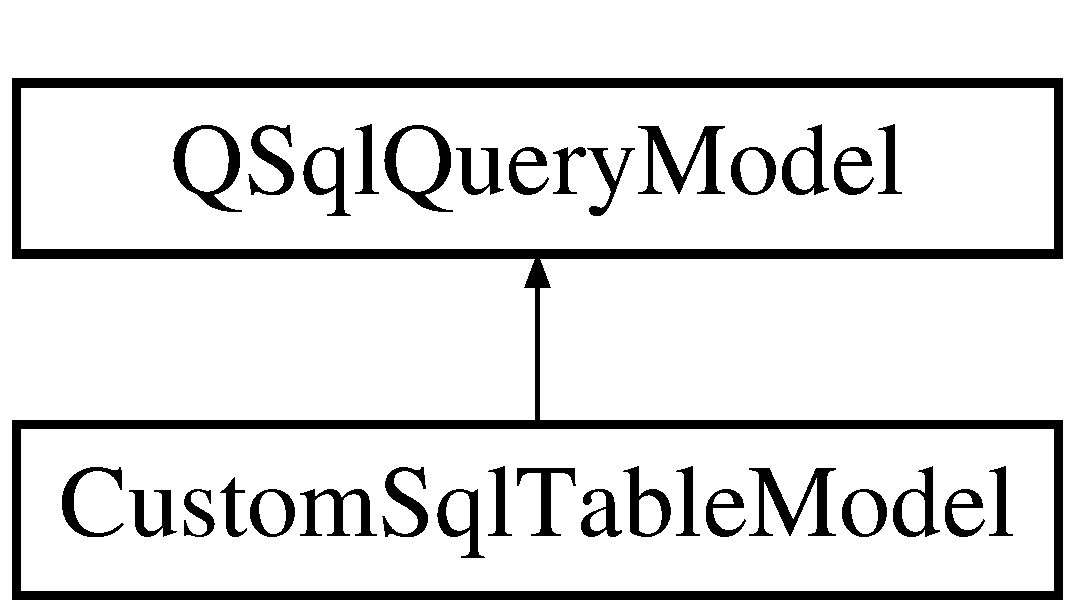
\includegraphics[height=2.000000cm]{class_custom_sql_table_model}
\end{center}
\end{figure}
\subsection*{Public Member Functions}
\begin{DoxyCompactItemize}
\item 
\mbox{\Hypertarget{class_custom_sql_table_model_a075e9fa54b6c339eedbc893c8c048ab0}\label{class_custom_sql_table_model_a075e9fa54b6c339eedbc893c8c048ab0}} 
{\bfseries Custom\+Sql\+Table\+Model} (Q\+Object $\ast$parent=nullptr)
\item 
\mbox{\Hypertarget{class_custom_sql_table_model_abff2c44cf6c27ee0a602b753a9f74c1b}\label{class_custom_sql_table_model_abff2c44cf6c27ee0a602b753a9f74c1b}} 
Qt\+::\+Item\+Flags {\bfseries flags} (const Q\+Model\+Index \&index) const
\item 
\mbox{\Hypertarget{class_custom_sql_table_model_ab6ea7405d3235fa32e223b7d8295c00d}\label{class_custom_sql_table_model_ab6ea7405d3235fa32e223b7d8295c00d}} 
bool {\bfseries set\+Data} (const Q\+Model\+Index \&index, const Q\+Variant \&value, int)
\end{DoxyCompactItemize}


The documentation for this class was generated from the following files\+:\begin{DoxyCompactItemize}
\item 
customsqltablemodel.\+h\item 
customsqltablemodel.\+cpp\end{DoxyCompactItemize}

\hypertarget{class_custom_table_model}{}\section{Custom\+Table\+Model Class Reference}
\label{class_custom_table_model}\index{Custom\+Table\+Model@{Custom\+Table\+Model}}
Inheritance diagram for Custom\+Table\+Model\+:\begin{figure}[H]
\begin{center}
\leavevmode
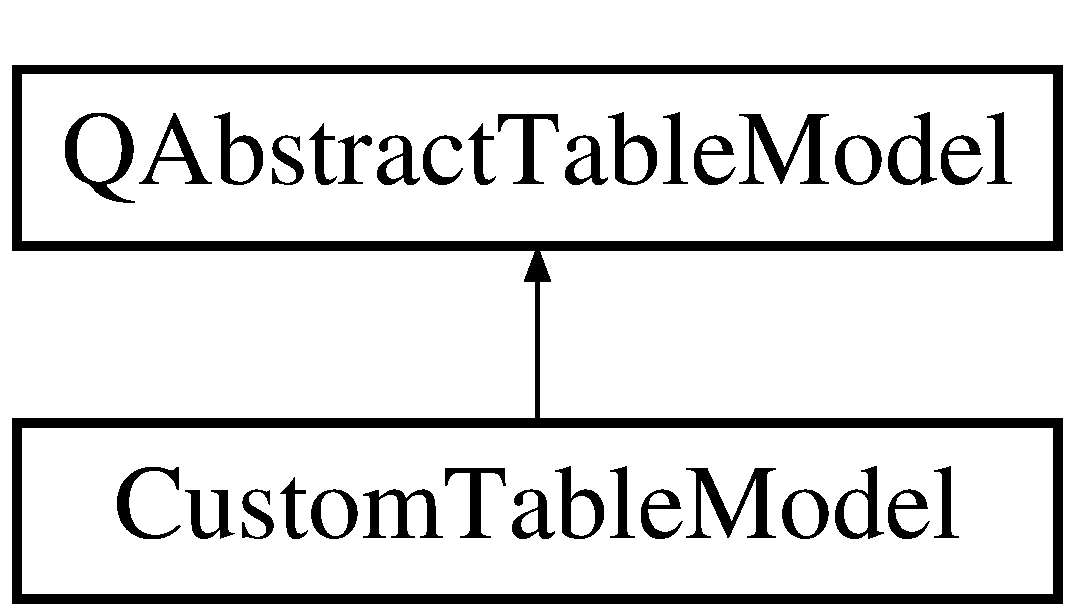
\includegraphics[height=2.000000cm]{class_custom_table_model}
\end{center}
\end{figure}
\subsection*{Public Member Functions}
\begin{DoxyCompactItemize}
\item 
\mbox{\Hypertarget{class_custom_table_model_a7a3b36ca24291f821f064a733ce4a5d3}\label{class_custom_table_model_a7a3b36ca24291f821f064a733ce4a5d3}} 
{\bfseries Custom\+Table\+Model} (Q\+Object $\ast$parent, Q\+String\+List \&column\+\_\+names, Q\+String\+List \&types)
\item 
\mbox{\Hypertarget{class_custom_table_model_a3c0eeb384e13eeddf21ad37f9bc1c565}\label{class_custom_table_model_a3c0eeb384e13eeddf21ad37f9bc1c565}} 
{\bfseries Custom\+Table\+Model} (Q\+Object $\ast$parent, Q\+String\+List \&column\+\_\+names)
\item 
\mbox{\Hypertarget{class_custom_table_model_a494801afcf3c25ca9befd159fb32527d}\label{class_custom_table_model_a494801afcf3c25ca9befd159fb32527d}} 
virtual int {\bfseries row\+Count} (const Q\+Model\+Index \&rc\+Parent=Q\+Model\+Index()) const
\item 
\mbox{\Hypertarget{class_custom_table_model_a50a175468f40478f75d84caf0f341b20}\label{class_custom_table_model_a50a175468f40478f75d84caf0f341b20}} 
virtual int {\bfseries column\+Count} (const Q\+Model\+Index \&rc\+Parent=Q\+Model\+Index()) const
\item 
\mbox{\Hypertarget{class_custom_table_model_a7dec8d4c9b036b46d8e5ba045fa245bf}\label{class_custom_table_model_a7dec8d4c9b036b46d8e5ba045fa245bf}} 
virtual Q\+Variant {\bfseries data} (const Q\+Model\+Index \&index, int role=Qt\+::\+User\+Role) const
\item 
\mbox{\Hypertarget{class_custom_table_model_ac7cc493ed26bdb34beacd82fc4565371}\label{class_custom_table_model_ac7cc493ed26bdb34beacd82fc4565371}} 
virtual bool {\bfseries set\+Data} (const Q\+Model\+Index \&index, const Q\+Variant \&value, int role=Qt\+::\+User\+Role)
\item 
\mbox{\Hypertarget{class_custom_table_model_a59aa7112f03780da11d4cb4163d9c79d}\label{class_custom_table_model_a59aa7112f03780da11d4cb4163d9c79d}} 
virtual Q\+Variant {\bfseries header\+Data} (int n\+Section, Qt\+::\+Orientation n\+Orientation, int n\+Role=Qt\+::\+User\+Role) const
\item 
\mbox{\Hypertarget{class_custom_table_model_a9be3af7745a5a8cd7a75fa7c9b5d81ba}\label{class_custom_table_model_a9be3af7745a5a8cd7a75fa7c9b5d81ba}} 
virtual Qt\+::\+Item\+Flags {\bfseries flags} (const Q\+Model\+Index \&index) const
\item 
\mbox{\Hypertarget{class_custom_table_model_a571c48faa96af1afa9dc2d8dfb90d709}\label{class_custom_table_model_a571c48faa96af1afa9dc2d8dfb90d709}} 
void {\bfseries clear} ()
\item 
\mbox{\Hypertarget{class_custom_table_model_a920879faea184930906ec569b5fcd185}\label{class_custom_table_model_a920879faea184930906ec569b5fcd185}} 
bool {\bfseries Is\+Empty} ()
\item 
\mbox{\Hypertarget{class_custom_table_model_aa2a289578ed7fd2322a015e95dd5e0d3}\label{class_custom_table_model_aa2a289578ed7fd2322a015e95dd5e0d3}} 
bool {\bfseries insert\+Rows} (int n\+Row, int n\+Count, const Q\+Model\+Index \&rc\+Parent=Q\+Model\+Index())
\item 
\mbox{\Hypertarget{class_custom_table_model_ab046cc94b91bf01a13ae9e67d6163488}\label{class_custom_table_model_ab046cc94b91bf01a13ae9e67d6163488}} 
bool {\bfseries remove\+Rows} (int row, int count, const Q\+Model\+Index \&parent\+\_\+index=Q\+Model\+Index())
\item 
\mbox{\Hypertarget{class_custom_table_model_a8381f4bba13a26063ca8b2f474081e91}\label{class_custom_table_model_a8381f4bba13a26063ca8b2f474081e91}} 
bool {\bfseries move\+Rows} (const Q\+Model\+Index \&rc\+Parent\+Source, int n\+Row\+Source, int n\+Count, const Q\+Model\+Index \&rc\+Parent\+Dest, int n\+Child\+Dest)
\item 
\mbox{\Hypertarget{class_custom_table_model_a684d28c48f5ef867640bb8b987fc8a72}\label{class_custom_table_model_a684d28c48f5ef867640bb8b987fc8a72}} 
bool {\bfseries append\+Row} (Q\+String\+List data)
\item 
\mbox{\Hypertarget{class_custom_table_model_ac842d36dd5b98e0419bf1c0f3e7a3da8}\label{class_custom_table_model_ac842d36dd5b98e0419bf1c0f3e7a3da8}} 
Qt\+::\+Drop\+Actions {\bfseries supported\+Drop\+Actions} () const
\item 
\mbox{\Hypertarget{class_custom_table_model_a440b90b538ecac68f84bfe2d81e84cd9}\label{class_custom_table_model_a440b90b538ecac68f84bfe2d81e84cd9}} 
Q\+List$<$ Q\+String\+List $>$ $\ast$ {\bfseries get\+Data} ()
\item 
\mbox{\Hypertarget{class_custom_table_model_ab2e2187982786411f177d136b08446ad}\label{class_custom_table_model_ab2e2187982786411f177d136b08446ad}} 
Q\+String\+List $\ast$ {\bfseries get\+Col\+Names} ()
\item 
\mbox{\Hypertarget{class_custom_table_model_adc28a889c76fb54d97e18a135b5f9f86}\label{class_custom_table_model_adc28a889c76fb54d97e18a135b5f9f86}} 
Q\+List$<$ Q\+Pair$<$ Q\+String, int $>$ $>$ $\ast$ {\bfseries get\+Col\+Types} ()
\item 
\mbox{\Hypertarget{class_custom_table_model_a7583eb136e76f5e8d73dc69803106c56}\label{class_custom_table_model_a7583eb136e76f5e8d73dc69803106c56}} 
void {\bfseries Determine\+Columns\+Types} ()
\end{DoxyCompactItemize}
\subsection*{Public Attributes}
\begin{DoxyCompactItemize}
\item 
\mbox{\Hypertarget{class_custom_table_model_af039586acef435fc4090b775101a3589}\label{class_custom_table_model_af039586acef435fc4090b775101a3589}} 
Q\+String\+List {\bfseries m\+\_\+column\+\_\+names}
\end{DoxyCompactItemize}
\subsection*{Protected Attributes}
\begin{DoxyCompactItemize}
\item 
\mbox{\Hypertarget{class_custom_table_model_a8ec6cce6f60343f187d5791ae342b8e3}\label{class_custom_table_model_a8ec6cce6f60343f187d5791ae342b8e3}} 
Q\+List$<$ Q\+Pair$<$ Q\+String, int $>$ $>$ {\bfseries m\+\_\+types}
\item 
\mbox{\Hypertarget{class_custom_table_model_ac8faea1ca0763add8fd5436de72fa22a}\label{class_custom_table_model_ac8faea1ca0763add8fd5436de72fa22a}} 
Q\+List$<$ Q\+String\+List $>$ {\bfseries m\+\_\+data}
\end{DoxyCompactItemize}


The documentation for this class was generated from the following files\+:\begin{DoxyCompactItemize}
\item 
customtablemodel.\+h\item 
customtablemodel.\+cpp\end{DoxyCompactItemize}

\hypertarget{class_main_window}{}\section{Main\+Window Class Reference}
\label{class_main_window}\index{Main\+Window@{Main\+Window}}
Inheritance diagram for Main\+Window\+:\begin{figure}[H]
\begin{center}
\leavevmode
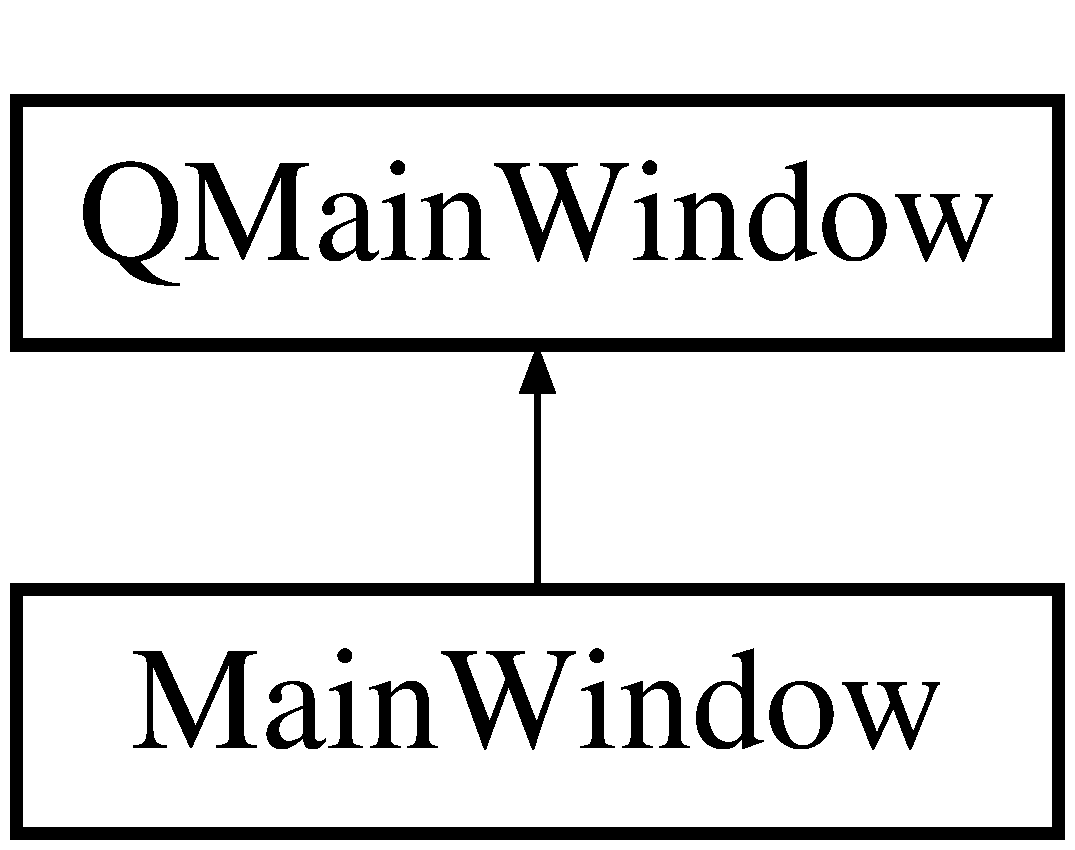
\includegraphics[height=2.000000cm]{class_main_window}
\end{center}
\end{figure}
\subsection*{Public Member Functions}
\begin{DoxyCompactItemize}
\item 
\mbox{\Hypertarget{class_main_window_a8b244be8b7b7db1b08de2a2acb9409db}\label{class_main_window_a8b244be8b7b7db1b08de2a2acb9409db}} 
{\bfseries Main\+Window} (Q\+Widget $\ast$parent=0)
\item 
\mbox{\Hypertarget{class_main_window_a45f35b5048fc97debcc8bd1cbd6f31cb}\label{class_main_window_a45f35b5048fc97debcc8bd1cbd6f31cb}} 
void {\bfseries check\+String} (Q\+String \&temp, Q\+Char character=0)
\item 
\mbox{\Hypertarget{class_main_window_a6bb6d76a07479f691ad0a416e71f2918}\label{class_main_window_a6bb6d76a07479f691ad0a416e71f2918}} 
void {\bfseries open\+C\+S\+V\+File} (const Q\+String \&file\+Name)
\item 
\mbox{\Hypertarget{class_main_window_a2b4b4a9321cf02d591d5217976a47664}\label{class_main_window_a2b4b4a9321cf02d591d5217976a47664}} 
bool {\bfseries save\+C\+S\+V\+File} (const Q\+String \&file\+Name)
\item 
\mbox{\Hypertarget{class_main_window_af61e44314f27379c620dd2e964fe3cb8}\label{class_main_window_af61e44314f27379c620dd2e964fe3cb8}} 
void {\bfseries open\+Sql} (const Q\+String \&file\+Name)
\item 
\mbox{\Hypertarget{class_main_window_ac27d646901950cb54a4116a69a042c6b}\label{class_main_window_ac27d646901950cb54a4116a69a042c6b}} 
void {\bfseries fill\+From\+Data} (const Q\+Abstract\+Table\+Model \&model, Q\+Sql\+Database \&data\+Base\+To\+Save, Q\+String table\+Name)
\item 
\mbox{\Hypertarget{class_main_window_a020d537dfc654cc707e94d290b30a611}\label{class_main_window_a020d537dfc654cc707e94d290b30a611}} 
void {\bfseries fill\+From\+Header} (const Q\+Abstract\+Table\+Model \&model, Q\+Sql\+Database \&data\+Base\+To\+Save, Q\+String table\+Name)
\item 
\mbox{\Hypertarget{class_main_window_a3c7c547487114c77ccfe82140a045ece}\label{class_main_window_a3c7c547487114c77ccfe82140a045ece}} 
Q\+String {\bfseries what\+Type\+Of\+Attribute} (const Q\+String \&str) const
\end{DoxyCompactItemize}


The documentation for this class was generated from the following files\+:\begin{DoxyCompactItemize}
\item 
mainwindow.\+h\item 
mainwindow.\+cpp\end{DoxyCompactItemize}

\hypertarget{class_save_to_sql_dialog}{}\section{Save\+To\+Sql\+Dialog Class Reference}
\label{class_save_to_sql_dialog}\index{Save\+To\+Sql\+Dialog@{Save\+To\+Sql\+Dialog}}
Inheritance diagram for Save\+To\+Sql\+Dialog\+:\begin{figure}[H]
\begin{center}
\leavevmode
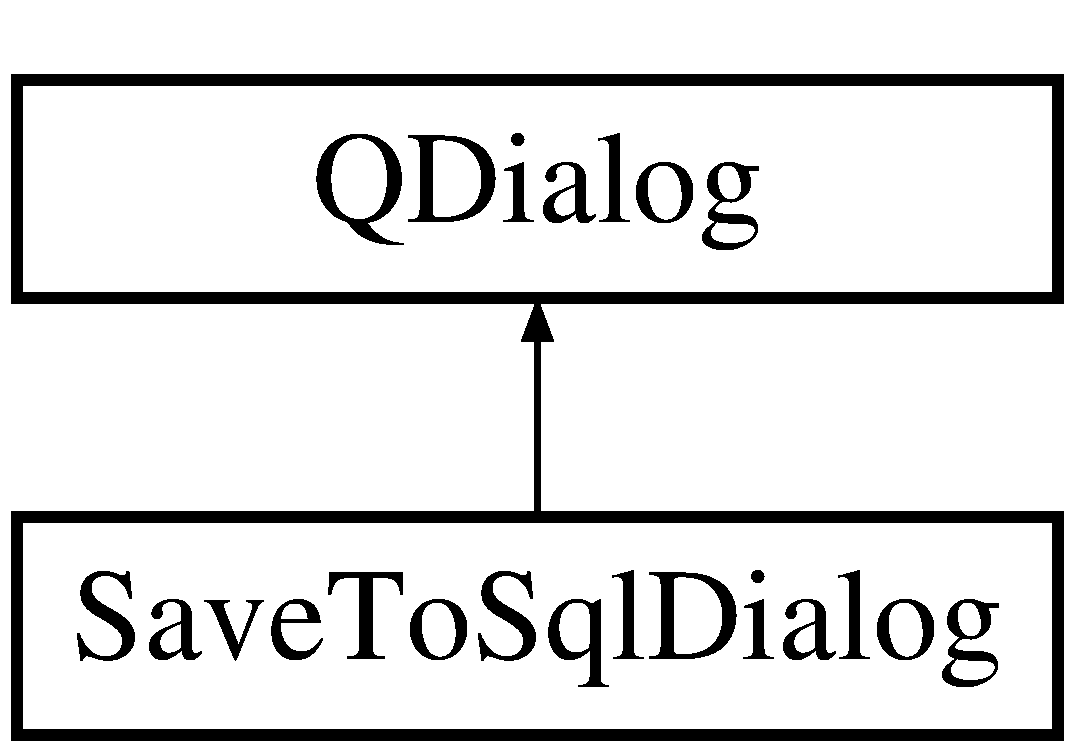
\includegraphics[height=2.000000cm]{class_save_to_sql_dialog}
\end{center}
\end{figure}
\subsection*{Public Member Functions}
\begin{DoxyCompactItemize}
\item 
\mbox{\Hypertarget{class_save_to_sql_dialog_a971f4d294b531372f14501f7b19d7e2e}\label{class_save_to_sql_dialog_a971f4d294b531372f14501f7b19d7e2e}} 
{\bfseries Save\+To\+Sql\+Dialog} (Q\+Widget $\ast$parent=0)
\item 
\mbox{\Hypertarget{class_save_to_sql_dialog_ada7a920c7005102fc334d709e1d2c18c}\label{class_save_to_sql_dialog_ada7a920c7005102fc334d709e1d2c18c}} 
Q\+String {\bfseries Get\+Data\+To\+Save} (Q\+Sql\+Database \&data\+Base)
\end{DoxyCompactItemize}


The documentation for this class was generated from the following files\+:\begin{DoxyCompactItemize}
\item 
savetosqldialog.\+h\item 
savetosqldialog.\+cpp\end{DoxyCompactItemize}

%--- End generated contents ---

% Index
\backmatter
\newpage
\phantomsection
\clearemptydoublepage
\addcontentsline{toc}{chapter}{Index}
\printindex

\end{document}
